
Lors de la navigation sur le Web, les internautes interagissent avec leur machine par le biais
des pages Web. Dans ce premier chapitre nous allons étudier \textsc{HTML} et \textsc{CSS}.\\
Le \textit{Worldwide Web} est apparu au \textsc{CERN} (Conseil Européen pour le Recherche Nucléaire) au début des années 90, à une époque où les 
principaux centre de recherche mondiaux étaient déjà connectés les un aux autres.\\
Pour faciliter les communications, le britannique Tim Berners-Lee et le belge Robert Cailliau mettent au point le \textit{système hypertexte} qui 
permet, à partir d'un document, d'en consulter d'autres en cliquant sur des mots-clés. Ces \textit{hyperliens} étaient souvent soulignés en bleu.
\begin{center}
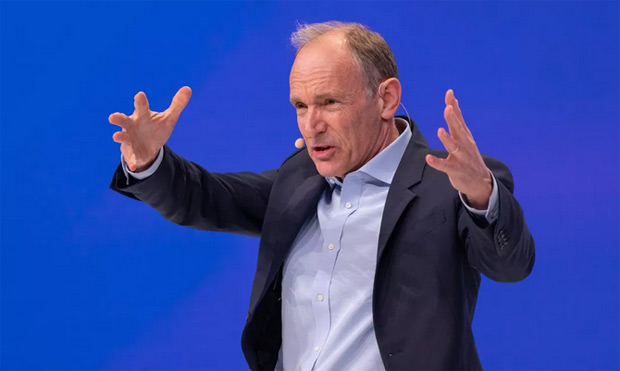
\includegraphics[height=4cm]{ch-web1/img/tbl.jpg}\hspace{3em}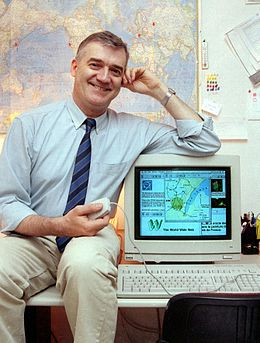
\includegraphics[height=4cm]{ch-web1/img/rc.jpg}\\
\scriptsize
Tim Berners-Lee (a gauche) et Robert Cailliau (à droite)
\end{center}
C'est également Tim Bernes-Lee qui développe le premier navigateur internet, ancêtre de \textsc{Firefox} et \textsc{Chrome}.
La première page web est toujours consultable à l'adresse \\\texttt{http://info.cern.ch/hypertext/WWW/TheProject.html}.\\

Techniquement, le web repose sur trois éléments :
\begin{itemize}
	\item	\textsc{HTTP} (\textit{HyperText Transfer Protocol}), le protocole de transmission des données \textit{via} un navigateur;
	\item 	des \textsc{URL} (\textit{Uniform Resource Locator}), chaines de caractères qui permettent d'identifier des ressources du web, telles des 
	sites. On les appelle aussi des \textit{adresses web};
	\item 	Le langage \textsc{HTML} (\textit{HyperText Markup Language}), qui permet de décrire le contenu des pages web.
\end{itemize}

\section{\textsc{HTML} : le descripteur}
	\picright{0.2}{ch-web1/img/html}{

	\textsc{HTML}  est un langage de balisage qui permet d'écrire des documents hypermédias, c'est-à-dire des documents contenant différents médias 
	(texte, image, son, vidéo) reliés les uns aux autres par des hyperliens.\\
	Il a beaucoup évolué depuis les années 90. La version la plus récente est \textsc{HTML5}.\\
	Un fichier \textsc{HTML} n'est qu'un simple fichier texte contenant des informations sur le contenu de la page à afficher.\\
    Les navigateurs web (\textsc{Chrome, Firefox, Safari, Internet Explorer}\ldots) se chargent (entre autres) de convertir les fichiers \textsc{HTML} en documents hypermédias.\\
}
Chaque navigateur possède ses spécificités, c'est pour cela que d'un navigateur à l'autre, le rendu d'une page peut différer.\\



	\textit{Grosso modo}, les informations sont

	\begin{itemize}
		\item 	soit entourées par une balise ouvrante et une balise fermante :
\begin{html}
\begin{minted}{html}
<em>Ce texte sera en italique</em>
\end{minted}
\end{html}
		\item 	soit contenues dans une balise orpheline :
\begin{html}
\begin{minted}{html}
<img src="image.jpg">
\end{minted}
\end{html}
	\end{itemize}

\begin{exercice}
	\begin{enumerate}
		\item 	Dans le répertoire \texttt{\textsc{HTML}5/} de la séance, ouvrir le fichier \texttt{index.html} et examiner son contenu (regarder la page 
		avec le 
		navigateur \textsc{Chrome}).
		\item 	Visualiser le code source \textsc{HTML} de cette page (\texttt{Ctrl+U} sous Chrome).
		\item 	Avec \textsc{PyCharm} ou \textsc{Notepad++} (par exemple), creér un fichier \textsc{HTML} reprenant l'ensemble des fonctionnalités de l'exemple. 
				Vous pouvez par exemple rédiger un (faux ?) CV ou une (fausse ?) « page perso ».\\
				Vous pourrez incorporer des médias \textit{libres de droit}. La page devra comporter au moins 
				\begin{itemize}
				\item 	du texte;
				\item 	une photo;
				\item 	un lien vers une deuxième page;
				\item	la deuxième page, qui permet de revenir à la première;
				\item 	un son ou une musique;
				\item 	une vidéo si les conditions de téléchargement le permettent.
				\end{itemize}
		\textbf{Utilisez le mémento.}
	\end{enumerate}
	Il faut se rendre à l'évidence :
	\begin{center}
	\textit{Sans mise en forme, le \textsc{HTML}, c'est laid !\\ \ }\\
	\end{center}
\end{exercice}
	
\section{CSS : le décorateur}

	\picleft{0.2}{ch-web1/img/css}{
	
	Le CSS (Cascading Style Sheets) est un langage informatique qui décrit la présentation des documents \textsc{HTML}. C'est avec lui que nous 
	allons mettre 
	en forme les pages.\\
	Lors de la réalisation d'une page web « classique »{} le principe est le suivant : le(s) fichier(s) \textsc{HTML} contien(nen)t l'information 
	et les 
	données essentielles au document,  le fichier CSS contient toutes les propriétés graphiques, esthétiques, de la page.}
	\begin{exercice}
Visiter le site \texttt{http://www.csszengarden.com/} et contempler (pas plus de cinq minutes) les différents \textit{designs} proposés.\\
Qu'est-ce qui change ? Qu'est-ce qui reste identique ?\\
Le code source \textsc{HTML} de la page change-t-il beaucoup ?
\end{exercice}
	
	
	Pour faire simple, nous allons écrire dans un fichier CSS les propriétés de polices, de taille, de couleur et de style qui vont s'appliquer à 
	chaque balise du document \textsc{HTML}. Puis, dans 
	le document \textsc{HTML}, nous allons faire référence à ce fichier CSS (appelé aussi feuille de style).
	
\begin{exercice}
	\begin{enumerate}
		\item 	Dans le répertoire \texttt{\textsc{HTML}5 et CSS3/} de la séance, ouvrir le fichier \texttt{index.html} et examiner son contenu et 
		particulièrement 
		la manière de faire référence à la feuille de style \texttt{style.css}.
		\item 	Visualiser le code source \textsc{HTML} (\texttt{Ctrl+U} sous \textsc{Chrome}).
		\item 	Avec \textsc{PyCharm} ou \textsc{Notepad++} ouvrir le fichier \texttt{style.css} et l'examiner.
		\item 	Créer une feuille de style simple pour les pages de l'exercice précédent.\\
	\end{enumerate}
		\textbf{Utilisez le mémento.}
\end{exercice}
\section{Annexe}

le fichier \texttt{memento.pdf} recense les principales balises \textsc{HTML} et styles CSS.\\
Il est issu du site \texttt{http://www.openclassrooms.com}

